
\section{Related Work}

According to Dimiter V. Dimitrov's paper ``Medical Internet of Things and Big Data in Healthcare'', ``The Internet of Things (IoT) is a network of physical devices and other items, embedded with electronics, software, sensors, and network connectivity, which enables these objects to collect and exchange data.''$^2$ The proliferation of the Medical Internet of Things (mIoT) represents a revolution in digital healthcare because it will enable doctors and hospital systems to streamline workflows, increase productivity, and provide higher data-backed quality of care. Dimitrov highlights numerous challenges for mIoT, including 5 key capabilities that leading platforms must enable: (1) Simple connectivity, (2) Easy device management, (3) Information ingestion, (4) Informative analytics, and (5) reduced risk. Of these challenges, my project attempts to improve device management and informative analytics by creating a feature of the IoT Inspector that will analyze real-time traffic flows from connected smart medical devices and inform the user of any potential privacy vulnerabilities should a device be leaking sensitive metadata. Specifically, Dimitrov specifies a need for an ``intuitive dashboard [that] makes it all easy to understand,'' and through a client-facing application such as IoT Inspector, users are able to easily visualize the status of their connected devices. 

One of the foundations for my research was Noah Apthorpe et al., ``A Smart Home is No Castle: Privacy Vulnerabilities of Encrypted IoT Traffic.''$^3$ Apthorpe observes that with the increasing prevalence of always-on IoT devices, ``Passive network observers, such as Internet service providers, could potentially analyze IoT network traffic to infer sensitive details about users.'' By analyzing metadata from four smart home devices (a Sense sleep monitor, a Nest Cam Indoor security camera, a WeMo switch, and an Amazon Echo), Apthorpe measured the correlation between traffic rates and user interaction. He showed that even when IoT traffic is encrypted, second order information such as device activity spikes reveal potentially sensitive user information that third parties and adversaries would find valuable. These concerns are compounded when the nature of the information is personal medical data instead of consumer behavior. Particularly because of the repetitive nature of medical tests, clearly defined patterns of user activity, such as daily blood sugar or blood pressure readings, reveal common medical conditions just from metadata alone. 

Apthorpe introduces a three-step strategy that a passive network observer could use ``to identify devices in a smart home and infer user behavior'' (3). First, an adversary must separate the device traffic into packet streams. This can be done by classifying packet conversations by the external IP address of the server communicating with the device, since the gateway router typically makes it difficult to divide outgoing traffic into sets based on IP addresses of the origin device. Second, an adversary must label streams by type of device by performing reverse DNS lookups to ``pair service IP's with device identifying domain names.'' Only once each device's traffic has been isolated, will an adversary be able to examine a device's traffic rate to infer user behavior of the device. For example, even though the Amazon Echo is an always-on device, queries are only made when the user interacts with the device.

In the process of examining a device's traffic, the most obvious determinant of confidentiality is encryption. Packets of data sent in the clear can be trivially intercepted by adversaries and network observers by separating traffic by IP address and protocol into streams and concatenating payloads to reassemble the original content. Even if plaintext data is compressed, it is still trivial to recover the original content by recovering the compressed message and attempting decompression using a limited number of widely used compression algorithms, such as bzip. In either scenario (plaintext or compressed), an adversary is privy to first order information. For example, if a blood sugar monitor calculates the blood sugar level from an inserted test strip and transmits the results upon completion to a paired phone or access point, then a network observer can learn the actual test results in addition to the frequency with which a particular user measures his blood sugar. Transmitting application data in the clear is a severe (and seemingly obvious) design flaw, and yet it is prevalent among IoT device manufacturers. In a recent Freedom to Tinker Post, Nick Feamster observes, ``many devices fail to encrypt at least some of the traffic that they send and receive. Investigating the traffic to and from these devices turned out to be much easier than expected, and many of the devices exchanged personal or private information with servers on the internet in the clear, completely unencrypted.''$^4$

Even when device traffic is encrypted, as in the case of the TLS or SSL protocols, adversaries can still learn a lot from transmitted metadata. However, due to the dense nature of packet data, it is not trivial to classify traffic as encrypted or plaintext. In ``Detecting encrypted traffic: a machine learning approach,'' Seunghun Cha et al. write, ``to identify encrypted traffic, the most widely used techniques are pattern matching in packet payloads and entropy analysis. $^5$ Entropy-based classification is the most common method to distinguish encrypted parts from plaintexts.'' Cha outlines a four-step methodology to determining encrypted versus unencrypted traffic:


\begin{enumerate}
  \item Separate each packet's header (non-encrypted) from its payload (potentially encrypted)
  \item Analyze randomness of payload using multiple tests, including Shannon Entropy, Chi-square, and arithmetic mean
  \item Use a training subset from plaintext protocols (HTTP, FTP, Telnet) and encrypted protocols (SSH, TLS) to determine a threshold entropy, above which indicates encrypted traffic
\end{enumerate}

I employ this approach as a baseline methodology for classifying traffic. A related problem is distinguishing encrypted traffic from compressed plaintext traffic, which is more difficult since compressed and encrypted traffic exhibit high orders of entropy. In this paper, I will restrict my focus to distinguishing plaintext traffic from encrypted traffic.  

\subsection{Problem Background}

Though the smart medical devices I examined in my study are intended for consumer home use, similar mIoT devices are increasingly being deployed in hospital environments and medical facilities to leverage systematic data collection and easily integrate readings and measurements into electronic health records. In these realms, mIoT devices are covered by the Security and Privacy rules of the Health Insurance Portability and Accountability Act of 1996 (HIPAA), which dictates core standards to protect sensitive patient information. According to a summary provided by the U.S. Department of Health and Human Services, the Security Rule Requires covered entities to maintain and appropriate administrative, technical, and physical safeguards for protecting electronic patient health information (e-PHI).$^6$ Specifically, covered entities must:

\begin{enumerate}
  \item Ensure the confidentiality, integrity, and availability of all e-PHI they create, receive, maintain, or transmit;
  \item Identify and protect against reasonably anticipated threats to the security or integrity of the information;
  \item Protect against reasonably anticipated, impermissible uses or disclosures; and
  \item Ensure compliance by their workforce. 
\end{enumerate}

Additionally, the Privacy Rule protects all individually identifiable health information held or transmitted by a covered entity or its business associate, in any form or media, whether electronic, paper or oral.$^7$ The Privacy Rule calls this information protected health information (PHI). Individually identifiable health information is information, including demographic data, that relates to:

\begin{enumerate}
  \item the individual's past, present or future physical or mental health or condition,
  \item the provision of health care to the individual, or
  \item the past, present, or future payment for the provision of health care to the individual,
\end{enumerate}

and that identifies the individual or for which there is a reasonable basis to believe it can be used to identify the individual. Individually identifiable health information includes many common identifiers (e.g., name, address, birth date, Social Security Number).

My research examines whether in the course of regular behavior, smart medical devices properly protect all individually identifiable health information as dictated by HIPAA. While the name of the user or patient may be protected, network observers and adversaries can see traffic being generated from each IP address. In an age where users are inseparable from their phones, an IP address is just as much a personal identifier as a social security number. By examining network traffic from an access point, it is possible to isolate traffic originating from a fixed set of IP addresses and subsequently mine the associated metadata for sensitive medical information.  

\section{Approach}

To examine metadata from a suite of mIoT devices, my research/project is divided into three main phases: 

\begin{enumerate}
  \item Data collection
  \item Deep packet inspection
  \item Representation through IoT Inspector
\end{enumerate}

\section{Implementation}

\subsection{Data Collection}

The first step in the data collection phase was to create an isolated test environment where I could connect various mIoT devices to a network and capture live traffic. Creating an isolated test environment was necessary because it enables me to easily separate traffic by device and filter out extraneous traffic on the network. To do this, I configured a Raspberry Pi to serve as a local access point (AP) or router, to which I would be able to connect my devices. Once my Raspberry Pi was running as a Wi-Fi router, I devised a systematic approach to collecting data. As part of my project, I chose four mIoT devices to inspect:

\begin{enumerate}
  \item Withings Wireless Blood Pressure Monitor
  \item Withings Body Composition Wi-Fi Scale
  \item 1byOne Digital Smart Wireless Body Fat Scale
  \item iHealth Ease Wireless Blood Pressure Monitor
\end{enumerate}

\begin{figure}
  \caption{Diagram of the data collection environment and data flow}
  \centering
    \fbox{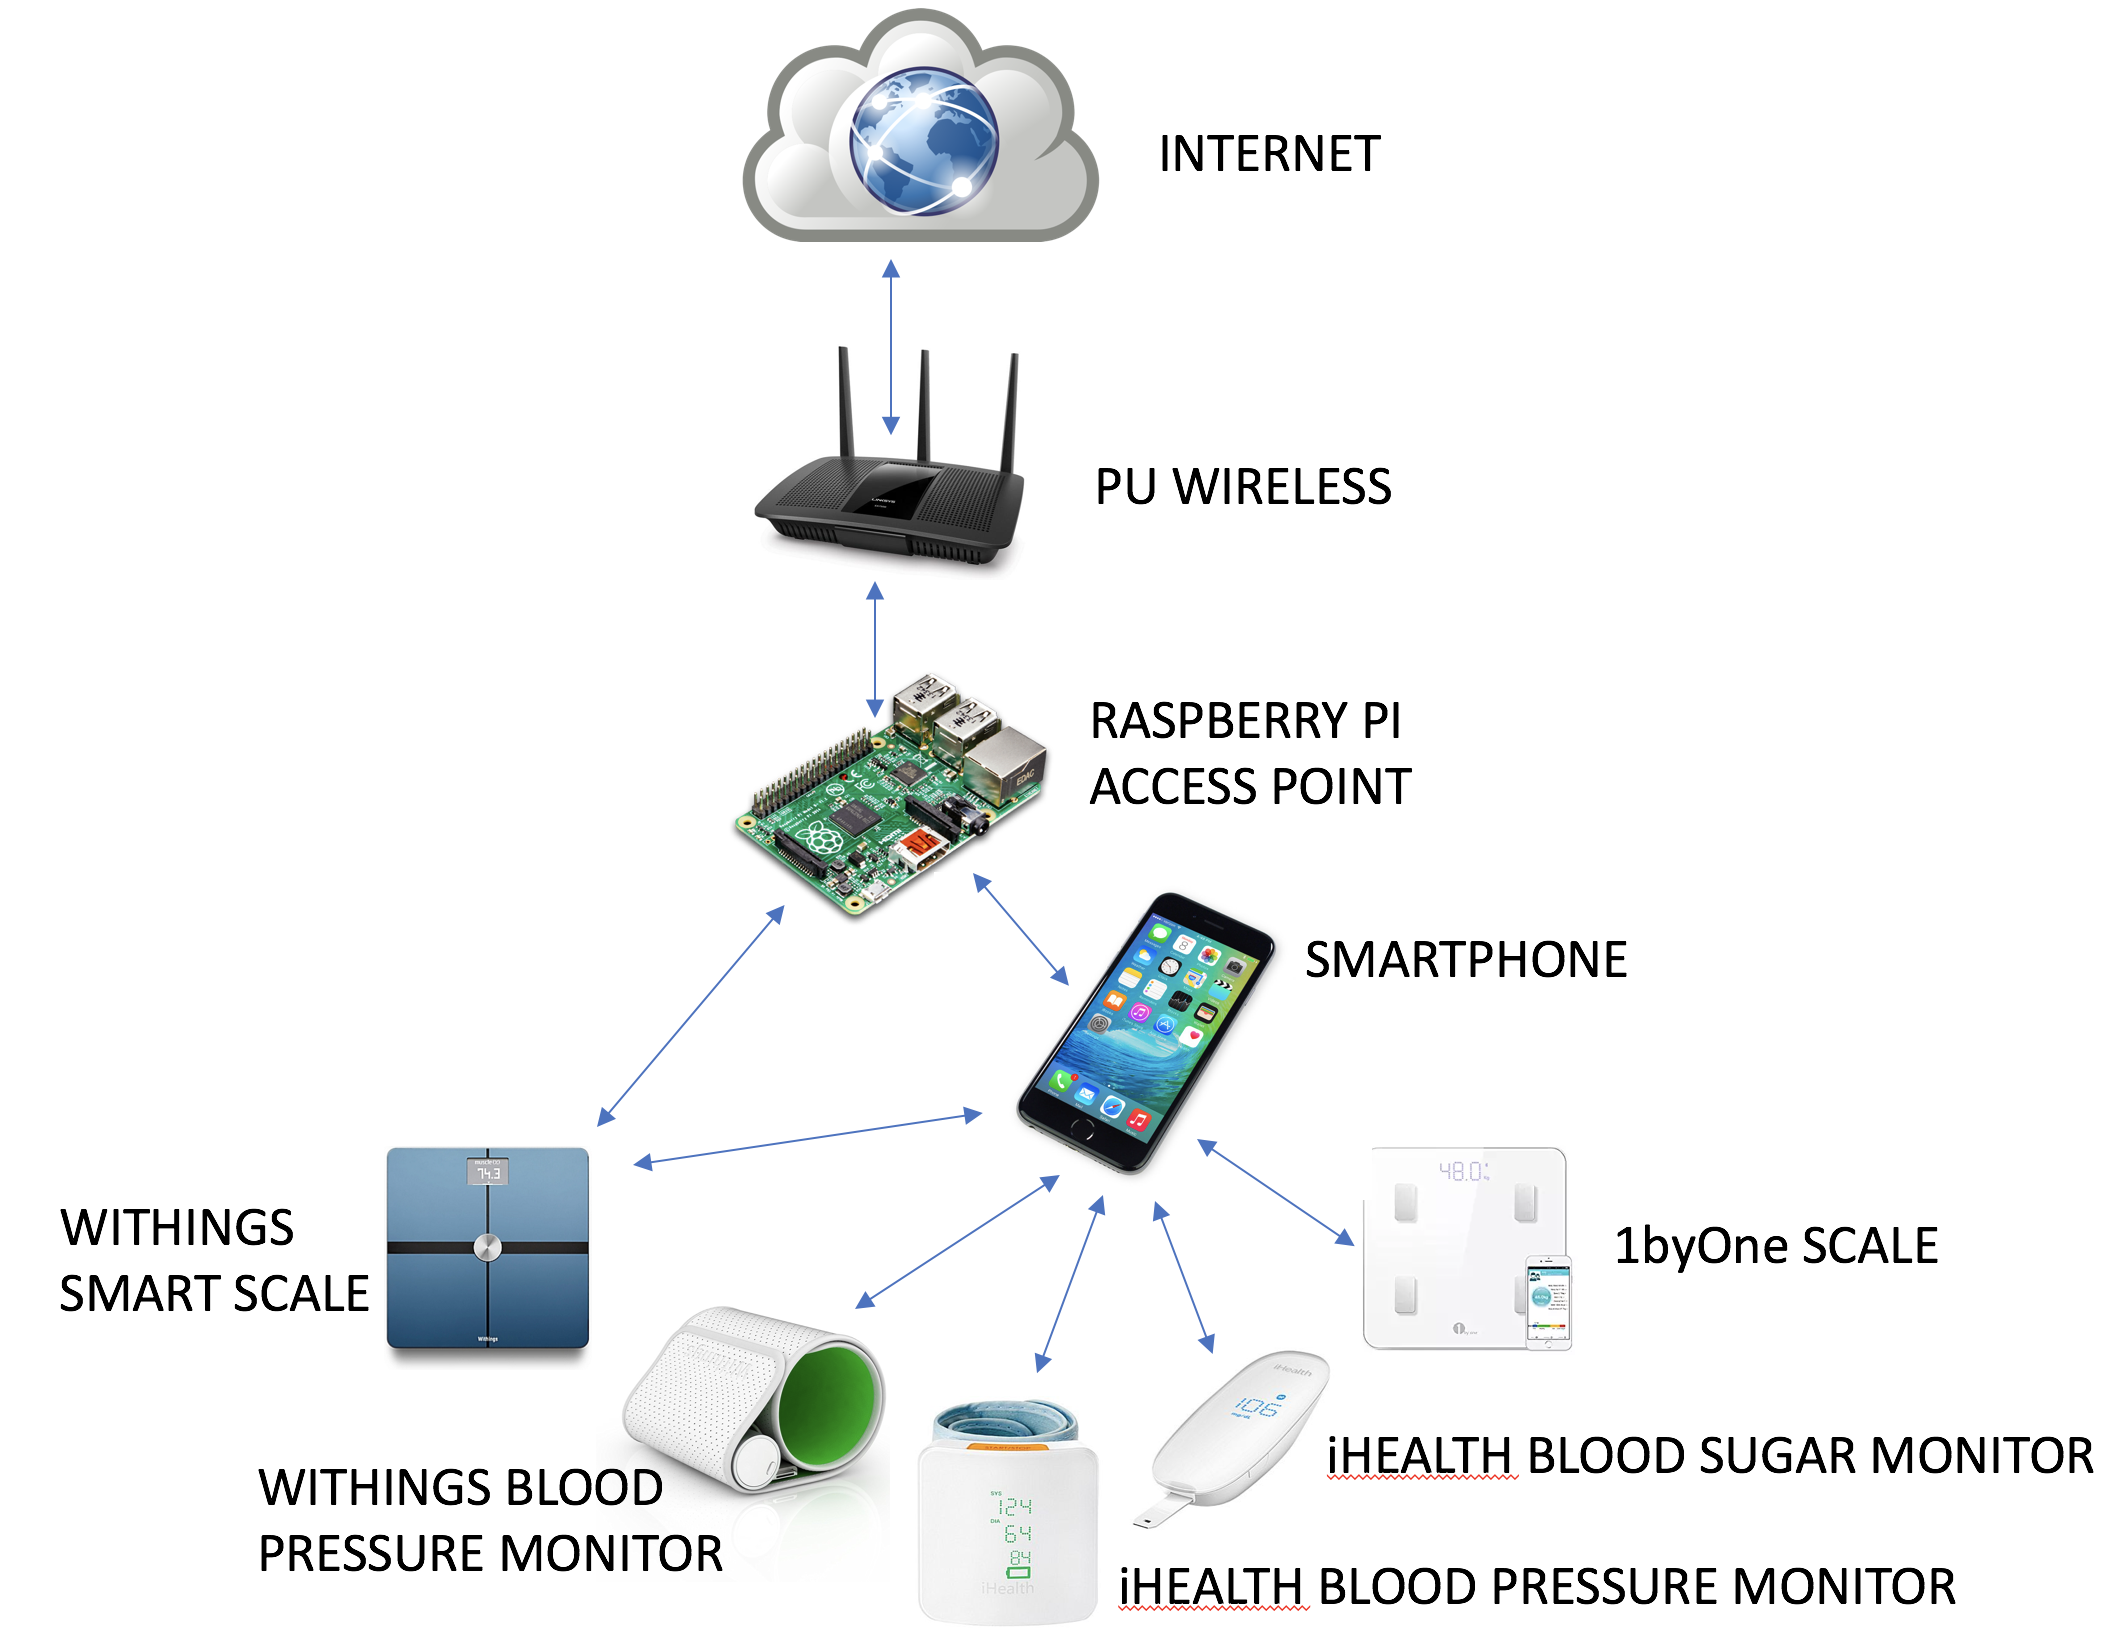
\includegraphics[scale=0.2]{network}}
\end{figure}

These devices are different from those analyzed in studies such as Apthorpe et al. because they are short-lived (i.e. only transmit data when in use for measuring blood pressure, weight, blood sugar, etc.). This provides intuitive frequency metadata and enables passive network observers to easily determine when a patient is using the device and how often. On the other hand, long-lived devices such as Amazon Echo or Nest are constantly transmitting data, though the number of packets sent increases substantially when the device is being actively used. I purposefully chose two smart scales and two blood pressure monitors so that I could compare the way in which different device manufacturers transmit application data and determine which company had better security or privacy practices, if any. 

In order to capture transmitted packets of data from the devices to the Pi, I used Wireshark to capture the Ethernet traffic being sent to the access point. I captured streams of data from each IoT device and saved it in the form of a PCAP file, which could be saved for offline analysis. When generating the dataset, I captured as many use cases of each device as possible, including user registration and sign-up, downloading patches and updates, vitals measurements, and health analytics. It is important not to ignore the use cases beyond general vitals measurement, because some of the most valuable information obtainable by an adversary would be a patch because it could reveal information about the way the embedded system in the device is designed. 

\subsection{Deep Packet Inspection}

The second phase in my project was deep packet inspection, in which I analyzed captured data streams from the suite of IoT devices for revealing metadata or unencrypted packets containing sensitive user information. I started by separating the steam of data by protocol, focusing mainly on HTTP and TCP packets and ignoring packets sent with SSL or TLS, as those are encrypted. Next I separated the payload, which contains application data, from the header of each packet for further analysis. 

The next step was to classify each incoming packet as either plaintext or encrypted. I experimented with three different schemes for this classification: naive ASCII approach, Shannon entropy test, and chi squared test. 

\subsection{Naive ASCII approach}
The first approach I used to determine whether a packet was plaintext or encrypted was the self-proposed naive ASCII approach. I simply examined each character in the payload as follows:


If all the characters in the payload are contained within the 128 character ASCII set, I anticipated that a packet would be unencrypted, since encrypted packets would need to contain characters from the extended ASCII set. While the naive ASCII approach does weed out encrypted packets, it does not identify all unencrypted packets, many of which contain characters from the extended ASCII set in addition to the printable characters. 

\subsection{Shannon Entropy Test}
The next approach I used to determine whether or not a packet was encrypted was the Shannon Entropy Test. This test calculates the entropy of each payload string, which is a quantitative measure of the variability in the frequency of the different possible characters. While random (or in this case, encrypted) strings have very high entropy, unencrypted plaintext and English strings exhibit fairly low entropy. This is because most characters are drawn from the limited set of printable characters and in English, many letters are much more likely to appear than others. For example, the letter e appears roughly 12.5\% of the time, while the letter $j$ appears less than 0.2\% of the time. To calculate the Shannon Entropy of a string, let $X$ be a random variable that takes on possible values $x_1$, $x_2$, ..., $x_n$. $p(x_i)$ is the probability that $X = x_i$:

$$H(X) = - \sum_{i = 1}^{n} p(x_i) log p(x_i)$$

\subsection{Chi Squared Test}
Lastly, the Chi Squared test compares the frequency of each character with its expected value from a uniform distribution. The value $x^2$ is calculated according to the formula:

$$X^2 = \sum_{i=1}^{n} \frac{(o_i-e_i)^2}{e_i}$$

The more a set of frequencies deviates from its expected values, the higher the value of $x_2$, and if the observed frequencies equal the expected frequencies then $x^2$ is 0. Therefore, English plaintext is expected to have a much higher deviation of character frequencies from the expected frequency (a uniformly random distribution). By setting the threshold value $x^2 = 1500$, I was able to effectively weed out the unencrypted payloads from those that were encrypted. In order to determine which of the three methods (naive ASCII, Shannon Entropy, or Chi Squared) yielded the most accurate classification of unencrypted packets, I ran a comparative analysis with five PCAP files with over 75,000 packets. From this analysis, I concluded that the most accurate encryption detection method would be Shannon Entropy. 

The selection of the Shannon Entropy test is supported by Cha et al., who write, ``Entropy-based classification is the most common method to distinguish encrypted parts from plaintexts,'' though it is only reasonable to do so under a threshold level of traffic due to the runtime of the algorithm.$^5$ Lyda and Hamrock ``used entropy analysis to identify encrypted and packed malware, but they only focused on offline executable files.''

\subsection{Dictionary Analysis}
Once I was able to identify plaintext packets, I identified potentially sensitive personal medical/personal identifying information by searching each string in the plaintext payload in several dictionaries. I used three dictionaries: a list of the 100 most common medical terms/conditions, a list of the most popular first male and female names, and a list of the most common personal identifying information (i.e. passport number, license, name, address, etc.). For my analysis of medical information leaks, I focused exclusively on the first and last of the three dictionaries, though for the IoT Inspector feature, I searched through all three dictionaries to mine for any potentially sensitive information that the user should be aware of that is being transmitted in the clear to the router. 

\subsection{Representation Through IoT Inspector}
The final component of my independent work was to design a representation of my findings so that an average inexperienced consumer of a smart device could become aware of breaches of confidentiality during regular device usage. Combining my research with Rohan Doshi and Gudrun Jonsdottir, we developed IoT Inspector, a smart home interface for users to visualize the potential vulnerabilities in their IoT devices.

IoT Inspector has three components: (1) default password protection, (2) confidentiality awareness, and (3) anomaly detection. The hub acts as a Wi-Fi access point; users simply connect their devices to the hub and visualize the status of their devices by navigating to the Connected Devices Dashboard which is running on a server on the hub. We implemented our hub by running the three component processes on a Raspberry Pi, which we outfitted to serve as a Wi-Fi access point to capture and analyze the transmitted data from each device. 

 Default password protection, implemented by Gudrun Jonsdottir, works by scanning the ports of the connected devices on the smart hub network and attempting to access each device using brute force and dictionary attacks with default passwords used by the Mirai botnet attack. If a default password is detected, the password is changed to a secure randomly generated string, which is displayed on the dashboard and emailed to the user. I implemented the confidentiality awareness component by alerting the user of any sensitive personal identifying information that is sent in plaintext from any of the devices connected to the smart hub, in response to the observation that device manufactures sometimes send user data or even entire patches in the clear using HTTP. Lastly, Rohan Doshi implemented anomaly detection by creating a machine learning model that learns a user's traditional device usage pattern and alerts the user if there is serious anomalous behavior, as would be observed if a connected device were to be controlled by an adversarial botnet in a DDoS attack. 

\section{Results}

After conducting deep packet analysis on each of the IoT devices, I found that there was very large variability in the methods each device used to send application data through the network when registering users, sending patches and updates, measuring vitals, or retrieving health analytics. All of the devices used encryption and protocols such as TLS or SSH to send sensitive first order information, such as the user's actual weight or blood sugar levels. However, there were various degrees of leaking second order information and metadata, scraped from sources such as HTTP GET requests, packet header information, and device conversation IP tables. Of the devices that I captured traffic for, the most secure implementation was the 1byOne Digital Smart Wireless Body Fat Scale. This device not only used encrypted protocols to deliver application data, but also masked names of packet destinations, unlike the Withings devices. 

The Withings Blood Pressure Monitor, out of all the devices I monitored, exhibited the most number of vulnerabilities when it comes to revealing sensitive user information during data transmission. I was able to capture enough sensitive second order data and metadata from a stream of traffic from the device in the course of typical usage to determine that the user of the device was measuring his or her blood pressure, and how frequently as well. 

First of all, it is very easy for a network observer to detect that a Withings IoT device is in use, because the information sections of all queries and responses to the Withings servers are titled with the brand of the device in the URL. This would make it exceptionally easy for a network observer to track all traffic originating from IP addresses querying an address such as static.withings.com. Because of the limited capabilities of medical IoT devices, as opposed to devices such as Amazon Echo, which can reach any endpoint on the Internet, there is a limited number of endpoints that are queried from each device. Figure 2 lists the queries made from the Withings Blood Pressure Monitor, along with their IP addresses. 

\begin{figure}
  \caption{Table of source and destination IP addresses}
  \begin{center}
    \begin{tabular}{||c c c||} 
    \hline
    Source IP & Dest IP & Information \\ [0.5ex] 
    \hline\hline
    $172.24.1.77$ & $224.0.0.251$ & withings-aura-bridge.tcp.local \\ 
    \hline
    $172.24.1.77$ &  $172.24.1.1$ & scalews.withings.net \\
    \hline
    172.24.1.1 &  172.24.1.77 & scalews.withings.net \\
    \hline
    172.24.1.77 &  172.24.1.1 & maintws.withings.net \\
    \hline
    172.24.1.77 &  172.24.1.1 & static.withings.com \\
    \hline
    172.24.1.1 &  172.24.1.77 & static.withings.com \\
    \hline
    172.24.1.1 &  172.24.1.77 & maintws.withings.net \\ [1ex] 
    \hline
    \end{tabular}
  \end{center}
\end{figure}

Even more concerning, I observed that one of the signature characteristics of the Withings Blood Pressure Monitor traffic was the fact that each reading concluded with a GET request for a stock photo of a person using the Withings Blood Pressure Monitor. If a picture is 1000 words, then this GET request is most certainly a cause for concern, as any adversary monitoring the traffic would be able to immediately determine when a user has finished measuring his or her blood pressure. This GET request is sent completely in the clear, and furthermore, it is not even displayed on the user interface of the app to the user of the device! It appears that there is no purpose of sending this image upon the success of each blood pressure reading, except inadvertently notifying network observers that the Withings Blood Pressure Monitor is in use. 

\begin{figure}
  \caption{Captured HTTP Packet reveals nature of device/user behavior}
  \centering
    \fbox{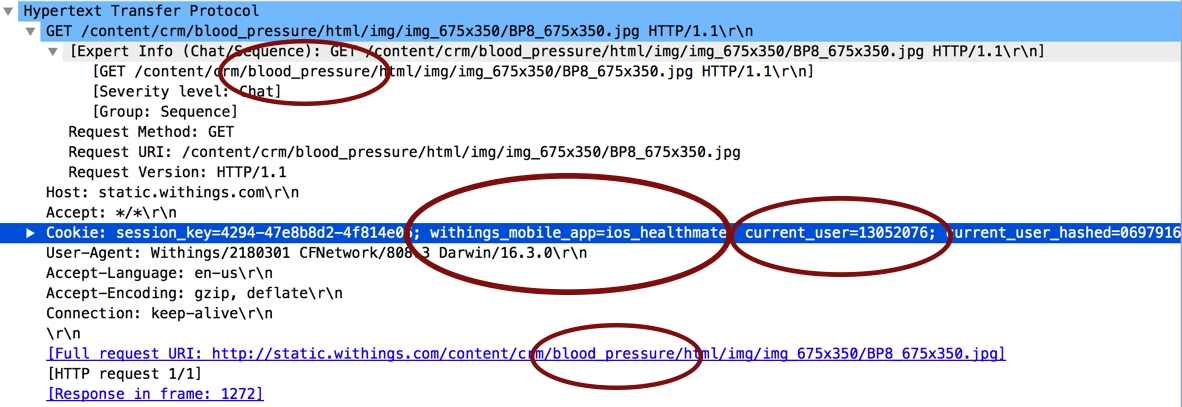
\includegraphics[scale=0.4]{bloodpacket}}
\end{figure}

In Figure 3, you can see that one packet alone reveals four sources of valuable information about the device. The plaintext string ``blood\textunderscore pressure'' appears twice, along with the string ``withings\textunderscore mobile\textunderscore app=ios\textunderscore healthmate''. Lastly, the ``current\textunderscore user'' field, while not directly disclosing the name of user, is potentially a unique identifier that associates that user with the subsequent blood pressure data. By monitoring this traffic for a period of time with many users, it would be trivial to match each packet of transmitted application data to the associated user. 

\begin{figure}
  \caption{Captured HTTP Packet reveals nature of device/user behavior}
  \centering
    \fbox{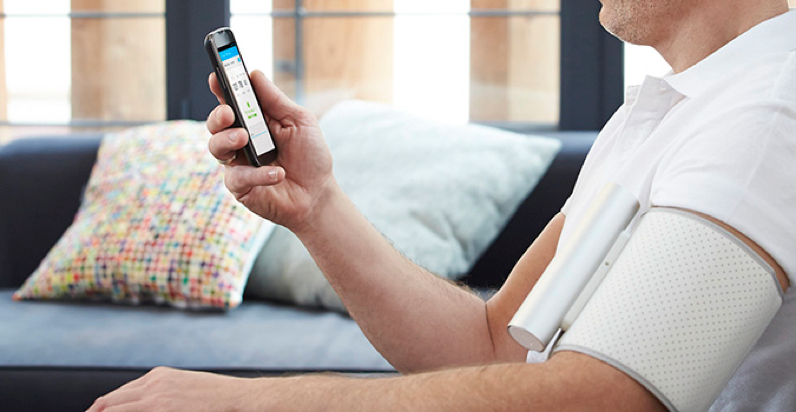
\includegraphics[scale=0.5]{bloodpressure}}
\end{figure}

In sharp contrast to the Withings Blood Pressure Monitor, the 1byOne Smart Scale was actually very secure. After pairing the scale with my smartphone and connecting to the test network to capture the transmitted packets, I found that the Smart Scale actually used TLSv1.2 on port 443 to send encrypted application data. Additionally, even though the scale only transmits data when it is being used to measure weight, the traffic is not trivial to detect without knowing the exact source IP address, as the packets are not labeled with revealing information about the nature of the device, and the destination addresses are not readable URLs such as the case of the Withings Blood Pressure Monitor. 

Therefore, when I ran my deep packet analysis on the traffic on the 1byOne Smart Scale, I was not able to compile information about the user's behavior in the same way as the blood pressure monitor. 
